\documentclass{book}
\usepackage{amsmath}
\usepackage{amsthm}
\usepackage{amsfonts}
\usepackage{chngcntr}
\usepackage{caption}
\usepackage{bm}
\usepackage[usenames,dvipsnames]{xcolor}
\usepackage{tikz}
\usepackage{hyperref}

\hypersetup{
    colorlinks,
    linkcolor={red!30!black},
    citecolor={blue!50!black},
    urlcolor={blue!80!black}
}

\counterwithout{section}{chapter}
\renewcommand{\thesubsection}{\Alph{subsection}}
\numberwithin{equation}{section}
\renewcommand{\theequation}{\arabic{equation}}
\renewcommand{\thefigure}{\arabic{figure}}

\theoremstyle{plain}
\newtheorem{thm}{Theorem}[section]
\newtheorem{lem}[thm]{Lemma} % same numbering with theorem
\newtheorem{prop}{Proposition}
\newtheorem{cor}{Corollary}

\renewcommand{\thethm}{\arabic{thm}}

\newtheorem*{thm*}{Theorem}
\newtheorem*{lem*}{Lemma}
\newtheorem*{prop*}{Proposition}
\newtheorem*{cor*}{Corollary}

\theoremstyle{definition}
\newtheorem{defn}{Definition}[section]
\renewcommand{\thedefn}{\arabic{defn}}
\newtheorem*{defn*}{Definition}

\theoremstyle{remark}
\newtheorem{rem}{Remark}
\newtheorem*{rem*}{Remark}


\theoremstyle{remark}
\newtheorem{ex}{Example}
\newtheorem*{ex*}{Example}

\newtheorem{prob}{Problem}
\newtheorem*{prob*}{Problem}

\newtheorem{ans}{Answer}
\newtheorem*{ans*}{Answer}

% fix the arrow direction for tikz
\makeatletter
\def\pgf@plot@curveto@handler@finish{%
  \ifpgf@plot@started%
    \pgfpathcurvebetweentimecontinue{0}{0.95}{\pgf@plot@curveto@first}{\pgf@plot@curveto@first@support}{\pgf@plot@curveto@second}{\pgf@plot@curveto@second}%
  \fi%
}
\makeatother

% larger arrow
\tikzset{
  big arrow/.style={
    decoration={markings,mark=at position 1 with {\arrow[scale=4]{>}}},
    postaction={decorate},
    shorten >=0.4pt}}

\begin{document}

\definecolor{DarkBlue}{RGB}{0,0,64}
\definecolor{DarkBrown}{RGB}{64,20,10}
% annotation macros
\newcommand{\repl}[2]{{\color{gray} [#1] }{\color{blue} #2}}
\newcommand{\add}[1]{{\color{blue} #1}}
\newcommand{\del}[1]{{\color{gray} [#1]}}
\newcommand{\note}[1]{{\color{DarkBrown}\footnotesize \textsc{Note.} #1}}
\newcommand{\answer}[1]{{\color{DarkBlue}\footnotesize \textsc{Answer.} #1}}

\newcommand{\hl}[1]{{\color{red} #1}}

\tableofcontents


\part{NEWTONIAN MECHANICS}
\chapter{Experimental facts}

\section{The principles of relativity and determinancy}

\section{The galilean group and Newton's equations}

\section{Examples of mechanical systems}



\chapter{Investigation of the equations of motion}

\section{Systems with one degree of freedom}

\section{Systems with two degrees of freedom}

\section{Conservative force fields}

\section{Angular momentum}

\section{Investigation of motion in a central field}

\section{The motion of a point in three-space}

\section{Motions of a system of $n$ points}

\section{The method of similarity}

\part{LAGRANGIAN MECHANICS}

\chapter{Variational principles}

\section{Calculus of variations}

\section{Lagrange's equations}

\section{Legendre transformations}

\section{Hamilton's equations}

\section{Liouville's theorem}

\chapter{Lagrangian mechanics on manifolds}

\section{Holonomic constraints}

\section{Differentiable manifolds}

\section{Lagrangian dynamical systems}

\section{E. Noether's theorem}

\section{D'Alembert's principle}

\chapter{Oscillations}

\section{Linearization}

\section{Small oscillations}

\section{Behavior of characteristic frequencies}

\section{Parametric resonance}

\chapter{Rigid bodies}

\section{Motion in a moving coordinate system}

\section{Inertial forces and the Coriolis force}

\section{Rigid bodies}

\section{Euler's equations. Poinsot's description of the motion}

\section{Lagrange's top}

\section{Sleeping tops and fast tops}

\part{HAMILTONIAN MECHANICS}

\chapter{Differential forms}

\section{Exterior forms}

\section{Exterior multiplication}



\setcounter{subsection}{2}
%subsection C
\subsection{\label{sec:exterior_mapping}Behavior under mappings}


Let $f: \mathbb{R}^m \rightarrow \mathbb{R}^n$ be a linear map,
and $\omega^k$ an exterior $k$-form on $\mathbb{R}^n$.
Then there is a $k$-form $f^*\omega^k$ on $\mathbb{R}^m$,
whose value on the $k$ vectors $\pmb\xi_1, \dots, \pmb\xi_k \in \mathbb{R}^m$
is equal to the value of $\omega^k$ on their images:
$$
(f^*\omega^k)(\pmb\xi_1, \dots, \pmb\xi_k)
=
\omega^k(f\pmb\xi_1, \dots, f\pmb\xi_k).
$$

\setcounter{prob}{7}
\begin{prob}
  Verify that $f^*\omega^k$ is an exterior form.

\answer{Antisymmetry:
  $$
  \begin{aligned}
  (f^*\omega^k)(\pmb\xi_1, \dots, \pmb\xi_i, \dots, \pmb\xi_j, \dots, \pmb\xi_k)
  &=
  \omega^k(f\pmb\xi_1, \dots, f\pmb\xi_i, \dots, f\pmb\xi_j, \dots, f\pmb\xi_k)
  \\
  &=
  -\omega^k(f\pmb\xi_1, \dots, f\pmb\xi_j, \dots, f\pmb\xi_i, \dots, f\pmb\xi_k)
  \\
  &=
  -(f^*\omega^k)(\pmb\xi_1, \dots, \pmb\xi_j, \dots, \pmb\xi_i, \dots, \pmb\xi_k).
  \end{aligned}
  $$
}
\end{prob}

\begin{prob}
Verify that $f^*$ is a linear operator from the space of $k$-forms on $\mathbb R^n$
to the space of $k$-forms on $\mathbb R^m$
(the star \emph{superscript} means that $f^*$ acts in the opposite direction from $f$).

\answer{
  $$
  \begin{aligned}
  [f^*(\omega_1^k + \omega_2^k)](\pmb\xi_1, \dots, \pmb\xi_k)
  &=
  (\omega_1^k + \omega_2^k)(f\pmb\xi_1, \dots, f\pmb\xi_k)
  \\
  &=
  \omega_1^k(f\pmb\xi_1, \dots, f\pmb\xi_k)
  +\omega_2^k(f\pmb\xi_1, \dots, f\pmb\xi_k)
  \\
  &=
  (f^*\omega_1^k)(\pmb\xi_1, \dots, \pmb\xi_k)
  +
  (f^*\omega_2^k)(\pmb\xi_1, \dots, \pmb\xi_k).
  \end{aligned}
  $$
}
\end{prob}

\begin{prob}
  Let $f: \mathbb R^m \rightarrow \mathbb R^n$ and
  $g: \mathbb R^n \rightarrow \mathbb R^p$.
  Verify that $(g\circ f)^* = f^* \circ g^*$.

\answer{
  $$
  \begin{aligned}
  (g\circ f)^*\omega^k(\pmb\xi_1, \dots, \pmb\xi_k)
  &=
  \omega^k((g\circ f)\, \pmb\xi_1, \dots, (g\circ f)\, \pmb\xi_k)
  \\
  &=
  (g^*\omega^k)(f\pmb\xi_1, \dots, f\pmb\xi_k)
  \\
  &=
  (f^*\circ g^*) \, \omega^k(\pmb\xi_1, \dots, \pmb\xi_k).
  \end{aligned}
  $$
}
\end{prob}

\begin{prob}
  \label{prob:fstar_exprod}
Verify that $f^*$ preserves exterior multiplication:
$f^*(\omega^k \wedge \omega^l) = (f^*\omega^k) \wedge (f^*\omega^l).$

\answer{
  $$
  \begin{aligned}
  f^*(\omega^k\wedge \omega^l)(\pmb\xi_1, \dots, \pmb\xi_{k+l})
  &=
  (\omega^k\wedge \omega^l)(f\pmb\xi_1, \dots, f\pmb\xi_{k+l})
  \\
  &=
  \sum_{i}
  (\pm)
    \omega^k(f\pmb\xi_{i_1}, \dots, f\pmb\xi_{i_k}) \
    \omega^l(f\pmb\xi_{i_{k+1}}, \dots, f\pmb\xi_{i_{k+l}})
  \\
  &=
  \sum_{i}
  (\pm)
    (f^*\omega^k)(\pmb\xi_{i_1}, \dots, \pmb\xi_{i_k}) \
    (f^*\omega^l)(\pmb\xi_{i_{k+1}}, \dots, \pmb\xi_{i_{k+l}}).
  \\
  &=
    (f^*\omega^k \wedge f^*\omega^l)
    (\pmb\xi_{i_1}, \dots, \pmb\xi_{i_{k+l}}).
  \end{aligned}
  $$
}
\end{prob}


\section{Differential forms}

\section{Integration of differential forms}

\section{Exterior differentiation}


\chapter{Symplectic manifolds}


A symplectic structure on a manifold is a closed nondegenerate differential
2-form.  The phase space of a mechanical system has a natural symplectic
structure.

On a symplectic manifold, as on a riemannian manifold, there is a natural
isomorphism between vector fields and 1-forms.  A vector field on a symplectic
manifold corresponds to the differential of a function is called a
hamiltonian vector field.  A vector field on a manifold determines a phase
flow, i.e., a one-parameter group of diffeomorphisms.  The phase flow of a
hamiltonian vector field on a symplectic manifold preserves the symplectic
structure of phase space.

The vector fields on a manifold form a Lie algebra.  The hamiltonian
vector fields on a symplectic manifold also form a Lie algebra. The operation
in this algebra is called the Poisson bracket.

% section 37
\section{Symplectic structures on manifolds}

% subsection A
\subsection{Definition}



%\begin{defn*}
Let $M^{2n}$ be an even-dimensional differentiable manifold.
A \emph{symplectic structure} on $M^{2n}$ is a closed nondegenerate differential 2-form
$\omega^2$ on $M^{2n}$:
$$
d\omega^2 = 0
$$
and
$$
\forall \pmb \xi \ne 0
\quad
\exists \pmb \eta:
\;
\omega^2(\pmb \xi, \pmb \eta) \ne 0
\quad
(\pmb \xi, \pmb \eta \in TM_{\mathbf x}).
$$
The pair $(M^{2n}, \omega^2)$ is called
a \emph{symplectic manifold}.
%\end{defn*}

\begin{ex*}
  Consider the vector space $\mathbb R^{2n}$
  with coordinates $p_i, q_i$ and let
  $\omega^2 = \sum d p_i \wedge dq_i$.
\end{ex*}

\begin{prob*}
  Verify that $(\mathbb R^{2n}, \omega^2)$
  is a symplectic manifold.
  For $n = 1$ the pair $(\mathbb R^2, \omega^2)$
  is the pair (the plain, area).

\answer{
  Since $\omega^2 = d\omega^1$, with $\omega^1 = \sum_i p_i dq_i$,
  $d\omega^2 = dd\omega^1 = 0$ is closed.
  To show $\omega^2$ is degenerate, take a vector $\pmb\xi$,
  with at least one nonzero component, say it is $p_i$.
  Then, we construct another vector $\pmb\eta$ with $q_i = 1$,
  and other components being zeros.
  Obviously $\omega^2(\pmb\xi, \pmb\eta) = p_i \ne 0$.
  We can similarly show the case for a nonzero $q_i$ component.
  So the 2-form is nondegenerate.
}
\end{prob*}


The following example explains the appearance of symplectic manifolds
in dynamics.  Along with the tangent bundle of a differentiable manifold,
it is often useful to look at its dual--the cotangent bundle.

% subsection B
\subsection{The cotangent bundle and its symplectic structure}



Let $V$ be an $n$-dimensional differentiable manifold.
%
A 1-form on the tangent space to $V$ at a point $\mathbf x$ is called
a \emph{cotangent vector} to $V$ at $\mathbf x$.

This vector space of cotangent vectors is denoted by $T^*V_{\mathbf x}$,
called the \emph{cotangent space} to $V$ at $\mathbf x$.

The union of the cotangent spaces to the manifold at all of its points
is called the \emph{cotangent bundle}, and denoted by $T^*V$.
%
The set $T^*V$ has a natural structure of a differentiable manifold of
dimension $2 n$.
\note{Each point $\mathbf x \in V$ has a $n$-dimensional vectors space;
the dimensionality of $V$ is $n$}.
%
A point of $T^*V$ is a 1-form on the tangent space to $V$ at some point of $V$.
%
If $\mathbf q$ is a choice of a local coordinates for points in $V$,
then such a form is given by its $n$ components $\mathbf p$.
%
Together, the $2n$ numbers $\mathbf p, \mathbf q$ form a collection of local coordinates
for points in $T^*V$.


There is a natural projection
$f: T^*V \rightarrow V$.
\note{$f$ sends every 1-form on $TV_{\mathbf x}$
to the point $\mathbf x$}
%
The projection $f$ is differentiable and surjective.
\note{Each $\mathbf x \in V$ has at least one preimage on $T^*V$}
%
The preimage of a point $\mathbf x \in V$ under $f$
is the cotangent space $T^*V_{\mathbf x}$.


\begin{thm*}
The cotangent bundle $T^*V$ has a natural symplectic structure.
%
In the local coordinates described above,
the symplectic structure is given by the formula
$\omega^2 = d\mathbf p \wedge d\mathbf q = dp_1 \wedge dq_1 + \cdots + dp_n \wedge dq_n$.
\end{thm*}

\begin{proof}
First, we define a distinguished 1-form on $T^*V$.
%
Let $\pmb \xi \in T(T^*V)_p$ be a vector
\emph{tangent to the cotangent bundle at the point $p \in T^*V_{\mathbf x}$}
(Figure 166).
\note{This means $p$ is a 1-form with coordinates $\mathbf p$,
and we can express $\pmb \xi$ in local coordinates as $(d\mathbf p, d\mathbf q)$.}
%
The derivative $f_*: T(T^*V) \rightarrow TV$
of the natural projection $f: T^*V \rightarrow V$,
which takes $\pmb \xi$ to a vector $f_* \pmb \xi$ ($d\mathbf q$)
tangent to $V$ at $\mathbf x$.
%
We define a 1-form $\omega^1$ on $T^*V$ by the relation
$\omega^1(\pmb \xi) \equiv p( f_*\pmb \xi )$
\note{Remember that $p$ is a 1-form so it accepts
  a tangent vector $d\mathbf q = f_* \pmb \xi$
  as input and returns a number.}
%
In the local coordinates described above,
this form is
$\omega^1 = \mathbf p \cdot d\mathbf q$,
and
$\omega^2 = d\omega^1$ is nondegenerate.

\setcounter{figure}{165}
\begin{figure}
  \centering
  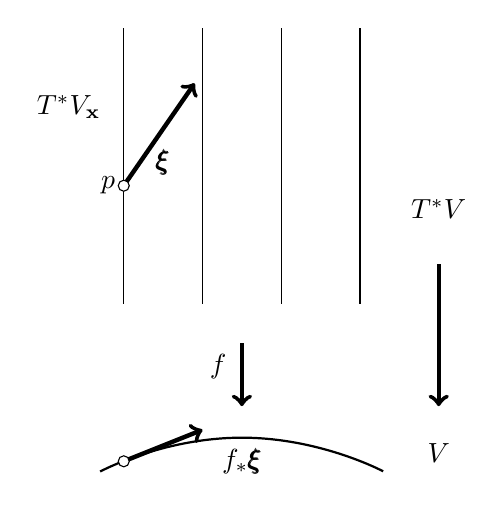
\begin{tikzpicture}
    % T^*V
    \draw [] (0, 2) -- (0, 5.5);
    \draw [] (1, 2) -- (1, 5.5);
    \draw [] (2, 2) -- (2, 5.5);
    \draw [] (3, 2) -- (3, 5.5);

    \node [] at (-0.7, 4.5) {$T^*V_{\mathbf x}$};

    % the mapping f
    \node [] at (1.2, 1.2) {$f$};
    \draw [ultra thick, ->] (1.5, 1.5) -- (1.5, 0.7);

    \node [] at (4.0, 3.2) {$T^*V$};
    \draw [ultra thick, ->] (4.0, 2.5) -- (4.0, 0.7);
    \node [] at (4.0, 0.1) {$V$};

    % vector xi
    \draw [ultra thick, ->] (0, 3.5) -- (0.9, 4.8);
    \node [] at (0.5, 3.8) {$\pmb\xi$};

    % point p
    \node [] at (-0.2, 3.5) {$p$};
    \draw [fill=white] (0, 3.5) circle (0.07);

    % V space

    \draw [thick] plot [smooth, tension=1]
      coordinates{(-0.3, -0.13) (1.5, 0.3) (3.3, -0.13)};
    \node [] at (1.5, 0) {$f_*\pmb\xi$};

    \draw [ultra thick, ->] (0, 0) -- (1.0, 0.4);
    \draw [fill=white] (0, 0) circle (0.07);

  \end{tikzpicture}
  \label{fig:1form_cotangent}
  \caption{The 1-form $\mathbf p \, d\mathbf q$ on
    the cotangent bundle}
\end{figure}


\end{proof}

\begin{rem*}
Consider a lagrangian mechanical system with configuration manifold $V$
and lagrangian function $L$.
It is easy to see that the lagrangian ``generalized velocity''
$\dot{\mathbf q}$ is a tangent vector to the configuration manifold $V$,
and the ``generalized momentum''
$\dot{\mathbf p} = \partial L/\partial \dot{\mathbf q}$
is a cotangent vector.
Therefore, the ``$\mathbf p, \mathbf q$'' phase space of the lagriangian
system is the cotangent bundle of the configuration manifold.
The theorem above shows that the phase space of a mechanical problem
has a natural symplectic manifold structure.
%Let $L = L(\mathbf q, \dot{\mathbf q})$  be a Lagrangian.
%%
%Then, $\dot{\mathbf q}$ is a tangent vector;
%%
%$\mathbf p = \partial L/\partial \dot{\mathbf q}$
%is a cotangent vector.
%%
%The $\mathbf p, \mathbf q$ phase space of the Lagrangian system
%is the cotangent of the configuration manifold.
%%
%The above theorem shows that the phase space of
%a mechanical problem has a natural symplectic
%manifold structure.
\end{rem*}

\begin{prob*}
  Show that the Legendre transform does not depend on the coordinate system:
  it takes a fucntion $:TV \rightarrow \mathbb R$ on the tangent bundle
  to a function $H: T^*V \rightarrow \mathbb R$ on the cotangent bundle.


\answer{
  Consider a coordinate transform $\mathbf q = \mathbf q(\mathbf Q)$,
  $$
  \begin{aligned}
  H
  &= \sum_i \dot q_i\frac{ \partial L } { \partial \dot q_i } - L
  = \sum_{ijk}
    \dot Q_j \frac{\partial q_i}{\partial Q_j}
    \frac{ \partial Q_k } { \partial q_i }
    \frac{ \partial L } { \partial Q_k } - L \\
  &= \sum_{jk}
    \dot Q_j \delta_{jk}
    \frac{ \partial L } { \partial Q_k } - L
  = \sum_j \dot Q_j \frac{ \partial L } { \partial Q_j } - L.
  \end{aligned}
  $$
  Thus the hamiltonian function is the same in the two coordinates.
}
\end{prob*}

% subsection C
\subsection{Hamiltonian vector fields}



A Riemann structure on a manifold establishes an isomorphism between
the spaces of tangent vectors and 1-forms.
%
A symplectic structure establishes a similar isomorphism.


\begin{defn*}
%
To each vector $\pmb \xi$
tangent to a symplectic manifold $(M^{2n}, \omega^2)$
at point $\mathbf x$, we associate a 1-form $\omega^1_{\pmb \xi}$
on $TM_{\mathbf x}$ by the formula
$$
\omega^1_{\pmb \xi}(\pmb \eta) = \omega^2(\pmb \eta, \pmb \xi),
\quad \forall \pmb \eta \in TM_{\mathbf x}.
$$
\end{defn*}

\begin{prob*}
Show that the correspondence $\pmb \xi \rightarrow \omega^1_{\mathbf \xi}$
is an isomorphism between the $2n$-dimensional vector spaces of vectors
and of 1-forms.
\end{prob*}

\begin{ex*}
  In $\mathbb{R}^{2n}=\{(\mathbf p, \mathbf q)\}$
  we will identify vectors and 1-forms by using the euclidean structure
  $(\mathbf x, \mathbf x) = \mathbf p^2 + \mathbf q^2$.
  Then the correspondences $\pmb\xi \rightarrow \omega^1_{\pmb\xi}$
  determines a transformation
  $\mathbb{R}^{2n} \rightarrow \mathbb{R}^{2n}$.
\end{ex*}

\begin{prob*}
  Calculate the matrix of this transformation in the basis
  $\mathbf p,\mathbf q$.

\answer{
For $n = 1$,
$\omega^2 = \pmb \eta \wedge \pmb \xi = \eta_1 \xi_2 - \eta_2 \xi_1$.
Then
$\omega^1_{\pmb \xi}(\pmb \eta) = (\pmb \eta, \mathbf J^{-1} \pmb \xi)$,
where $\mathbf J^{-1}$ means a rotation of $-\pi/2$, where
$$
\mathbf J =
\left(
  \begin{array}{cc}
    0  & -1 \\
    1  & 0
  \end{array}
\right)
\qquad
\mathbf J^{-1} =
\left(
  \begin{array}{cc}
    0  & 1 \\
    -1 & 0
  \end{array}
\right),
$$
with the indices of $p$ and $q$ being $1$ and $2$, respectively
(the convention of this book).

For higher dimensions, we just replace $1$ by the $n\times n$
identity matrix $E$,
$$
\mathbf J =
\left(
  \begin{array}{cc}
    0  & -E \\
    E  & 0
  \end{array}
\right)
\qquad
\mathbf J^{-1} =
\left(
  \begin{array}{cc}
    0  & E \\
    -E & 0
  \end{array}
\right).
$$


Generally, we have
$$
\omega^1_{\pmb \xi}(\pmb \eta) = (\pmb \eta, \mathbf I^{-1} \pmb \xi)
=\eta' \mathbf J^{-1} \pmb\xi.
$$
with the prime``$'$'' denoting the transpose.

However, later in this book, the author will frequently use the result
$$
\omega^2(\pmb\eta,\pmb\xi) = (I\pmb\eta, \pmb\xi) = \pmb\eta'\mathbf J' \pmb\xi,
$$
for this case. This is not generally true.
It requires the isomorphism $I$ to be equivalent to a matrix multiplication
of the symplectic matrix $\mathbf J$, and $\mathbf J' = \mathbf J^{-1}$.

In general,
$\omega^1_{\pmb \xi}$ is represented by the vector $I^{-1} \pmb \xi$,
and a 1-form $\omega_1$ is represented by the vector $I\, \omega_1$.
}
\end{prob*}
%






We will denote by $I$ the isomorphism
$I: T^*M_{\mathbf x} \rightarrow TM_{\mathbf x}$
(from 1-forms to tangent vectors,
$\omega^1_{\pmb \xi} \rightarrow \pmb \xi$).
%
Now let $H$ be a function on a symplectic manifold $M^{2n}$.
%
Then $dH$ is a differential 1-form on $M$ and
for every point there is a tangent vector to $M$ associated to it.
%
In this way, we obtain a vector field $IdH$ on $M$.


\begin{defn*}
%
The vector field $IdH$ is called \emph{Hamiltonian vector field}.
%
$H$ is called the \emph{Hamiltonian function}.
\end{defn*}

\begin{ex*}
  If $M^{2n} = R^{2n} = {(\mathbf p, \mathbf q)}$,
  then we obtain the phase velocity field
  of Hamilton's canonical equation:
  $$
  \dot{\mathbf x} = I\,dH(\mathbf x)
  \Longleftrightarrow
  \dot{\mathbf p} = - \frac{\partial H }{ \partial \mathbf q}
  \mathrm{\quad and \quad}
  \dot{\mathbf q} = \frac{\partial H}{\partial \mathbf p}.
  $$
\note{In the above example,
the 1-form is represented by the vector
$\nabla H = \left(\frac{\partial H}{\partial \mathbf p},
\frac{\partial H}{\partial q}\right)^T$
to invert this vector to corresponding tangent vector we multiple it by $\mathbf J$
%
\[
\arraycolsep=3.0pt\def\arraystretch{1.5}
\mathbf J \cdot \nabla H
=
\left(
  \begin{array}{ccc}
    0 & -1 \\
    1 & 0
  \end{array}
\right)
\left(
  \begin{array}{ccc}
    \frac{ \partial H }{ \partial \mathbf p } \\
    \frac{ \partial H }{ \partial \mathbf q }
  \end{array}
\right)
=
\left(
  \begin{array}{ccc}
    -\frac{ \partial H }{ \partial \mathbf q } \\
    \frac{ \partial H }{ \partial \mathbf p }
  \end{array}
\right)
=
\left(
  \begin{array}{ccc}
    \dot{\mathbf p} \\
    \dot{\mathbf q}
  \end{array}
\right).
\]}
\end{ex*}


%section 38
\section{Hamiltonian phase flows and their integral invariants}

Liouville's theorem asserts that the phase flow
preserve the symplectic structure.
%
Poincar\'e found a whole series of differential forms
which are preserved by the hamiltonian flow.

%\subsection A
\subsection{Hamiltonian phase flows preserve the symplectic structure}

Let $(M^{2n}, \omega^2)$ be a symplectic manifold and
$H: M^{2n} \rightarrow \mathbb{R}$ a function.
Assume that the vector field $IdH$
corresponds to $H$ gives a 1-parameter group
of diffeomorphism: $g^t: M^{2n} \rightarrow M^{2n}$:
$$
\left.\frac{d}{dt}\right|_{t = 0}
= I dH(\mathbf x).
$$
This group $g^t$ is the hamiltonian phase flow with
hamiltonian function $H$.

\note{
A \emph{diffeomorphism} is an isomorphism of smooth manifolds.
It is a smooth invertible function that maps one differentiable manifold
to another.

Not all differentiable maps are diffeomorphism, because of the one-to-one requirement.
For example, $(x, y) \rightarrow (y^2 \sin x, y^2 \cos x)$ is not invertible.
}

\begin{thm}
A hamiltonian phase flow preserves the symplectic structure:
$$
(g^t)^* \omega^2 = \omega^2.
$$
\end{thm}

\note{The definition of $(g^t)^*$:
  $g^t$ applies to $\mathbf x$ or a tangent vector,
  $(g^t)^*$ applies to $\omega$.
  The definition of
  $[(g^t)^*\omega^2](\pmb\xi, \pmb\eta) \equiv \omega^2(g^t\pmb\xi, g^t\pmb\eta).$
  See details in Sec. 33C.}


In the case $n = 1$, $M^{2n} = \mathbb{R}^2$, this theorem says
that the phase flow $g^t$ preserves area (Liouville's theorem).
%
For the proof of this theorem, it is useful to introduce
the following notation.

Let $M$ be an arbitrary manifold,
$c$ a $k$-chain on $M$ and $g^t: M \rightarrow M$
a one-parameter family of differentiable mappings.
We will construct a $(k+1)$-chain $Jc$ on $M$,
which we will call the
\emph{track of the chain $c$ under the homotopy
$g^t$, $0 \le t \le \tau$}.
\note{Roughly, ``homotopy'' means time evolution.}


Let $(D, f, \mathrm{Or})$ be one of the cells in the chain $c$.
\note{$D$ is the domain, a convex polygon in $\mathbb{R}^k$,
  $f$ is a mapping from the euclidean space to the manifold $\mathbb{R}^k \rightarrow M$,
  $\mathrm{Or}$ is the orientation.
  See page 184, \S 35.D.}
%
To this cell will be associated a cell $(D', f', \mathrm{Or}')$
  in the chain $Jc$ where $D' = I\times D$ is the direct product
  of the interval of $0 \le t \le \tau$ and $D$;
  the mapping $f': D' \rightarrow M$ is obtained from
  $f: D \rightarrow M$ by the formula
  $f'(t, x) = g^t f(x)$;
  and the orientation $\mathrm{Or}'$ of the space $\mathbb{R}^{k+1}$
  containing $D'$ is given by the frame
  $\mathbf e_0, \mathbf e_1, \dots, \mathbf e_k$,
  where $\mathbf e_0$ is the unit vector of the $t$ axis,
  and $\mathbf e_1, \dots, \mathbf e_k$ is an oriented frame for $D$.


We could say that $Jc$ is the chain swept out by $c$
  under the homotopy $g^t$, $0 \le t \le \tau$.
  The boundary of the chain $Jc$ consists of ``end-walls''
  made up of the initial and final positions of $c$,
  and the ``side surfaces'' filled in by the boundary of $c$.
\note{Below, we want to prove that the integrals on the side surfaces
  vanishes, so is the integral on the volume enclosed by the tube.
  Then the integrals at the two end walls, which are opposite
  in the signs must add to zero.}

\setcounter{figure}{166}
\begin{figure}
\centering
  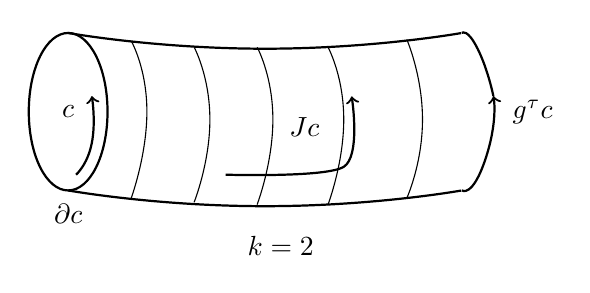
\begin{tikzpicture}
    % end-wall 1
    \draw [thick] plot [smooth cycle, tension=1]
      coordinates{(0, 0) (0.5, 1) (0, 2) (-0.5, 1)};
    % bottom of side surface
    \draw [thick] plot [smooth, tension=1]
      coordinates{(0, 0) (2.5, -0.2) (5, 0)};
    % top of the side surface
    \draw [thick] plot [smooth, tension=1]
      coordinates{(0, 2) (2.5,  1.8) (5, 2)};
    % end-wall 2
    \draw [thick, ->] plot [smooth, tension=1.5]
      coordinates{(5, 0) (5.3, 0.4) (5.4, 1.2)};
    \draw [thick] plot [smooth, tension=1.2]
    coordinates{(5.4, 1.2) (5.2, 1.8) (5, 2)};

    % intermediate rings
    \draw [] plot [smooth, tension=1]
      coordinates{(0.8, -0.1) (1.0, 1.0) (0.8, 1.9)};
    \draw [] plot [smooth, tension=1]
      coordinates{(1.6, -0.15) (1.8, 0.9) (1.6, 1.82)};
    \draw [] plot [smooth, tension=1]
      coordinates{(2.4, -0.18) (2.6, 0.9) (2.4, 1.82)};
    \draw [] plot [smooth, tension=1]
      coordinates{(3.3, -0.18) (3.5, 0.9) (3.3, 1.82)};
    \draw [] plot [smooth, tension=1]
      coordinates{(4.3, -0.1) (4.5, 0.9) (4.3, 1.92)};

    % dc
    \draw [->, thick] plot [smooth, tension=1]
      coordinates{(0.1, 0.2) (0.3, 0.6) (0.3, 1.2)};
    \node[](dc) at (0, -0.3){$\partial c$};

    % c
    \node[](c) at (0, 1.0){$c$};

    % J c
    \draw [->, thick] plot [smooth, tension=0.5]
      coordinates{(2, 0.2) (3.5, 0.3) (3.6, 1.2)};
    \node[](Jc) at (3, 0.8){$Jc$};

    % g c
    \node[](gc) at (5.9, 1.0){$g^\tau c$};

    % k = 2
    \node[](keq2) at (2.7, -0.7){$k = 2$};
  \end{tikzpicture}
%
  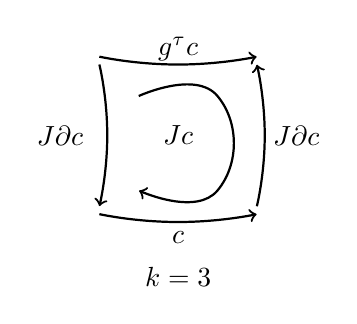
\begin{tikzpicture}
    % c
    \draw [thick, ->] plot [smooth, tension=1]
      coordinates{(0, 0) (1, -0.1) (2, 0)};
    \node[](c) at (1, -0.3){$c$};
    % g c
    \draw [thick, ->] plot [smooth, tension=1]
      coordinates{(0, 2) (1., 1.9) (2, 2)};
    \node[](gc) at (1, 2.1){$g^\tau c$};
    % J c, left
    \draw [thick, ->] plot [smooth, tension=1]
      coordinates{(0, 1.9) (0.1, 1) (0, 0.1)};
    \node[](Jcleft) at (-0.5, 1){$J\partial c$};
    % J c, right
    \draw [thick, ->] plot [smooth, tension=1]
      coordinates{(2, 0.1) (2.1, 1) (2, 1.9)};
    \node[](Jcright) at (2.5, 1){$J\partial c$};

    % the circle
    \draw [thick, ->] plot [smooth, tension=1.0]
      coordinates{(0.5, 1.5) (1.5, 1.5) (1.5, 0.3) (0.5, 0.3)};
    \node[](Jc) at (1, 1){$Jc$};
    % k = 3
    \node[](gc) at (1.0, -0.8){$k = 3$};
  \end{tikzpicture}
  \caption{Track of a cycle under homotopy.}
\end{figure}

It is easy to verify that under the choice of orientation made above
\begin{equation}
\partial (J c_k) = g^\tau c_k - c_k - J \partial c_k.
\label{eq:H_homotopy}
\end{equation}

\begin{lem*}
  Let $\gamma$ be a 1-chain in the symplectic manifold $(M^{2n}, \omega^2)$.
  Let $g^t$ be phase flow on $M$ with hamiltonian function $H$.
  Then
  $$
  \frac{d}{d\tau} \int_{J\gamma} \omega^2
  =
  \int_{g^\tau\gamma} dH.
  $$
\end{lem*}

\begin{proof}
  It is sufficient to consider a chain $\gamma$ with one cell
  $f: [0,1] \rightarrow M$.\note{$\gamma$ is a curve.}
  We introduce the notation
  $$
  \begin{aligned}
    f'(s, t) &= g^t f(s), \\
    \pmb\xi = \frac{ \partial f' } { \partial s },
    &\mathrm{\quad and \quad}
    \pmb\eta = \frac{ \partial f' } { \partial t }
    = TM_{f'(s, t)}.
  \end{aligned}
  $$
  By the definition of the integral,
  $$
  \int_{J\gamma} \omega^2
  =
  \int_0^1 \int_0^\tau \omega^2(\pmb\xi, \pmb\eta) \, dt \, ds.
  $$
  But the by the definition of the phase flow,
  $\pmb \eta$ is a vector (at the point $f'(s, t)$)
  of the hamiltonian flow with hamiltonian function $H$.
  \note{$\pmb\eta = I dH$.}
  By defintion of a hamiltonian field
  $\omega^2(\pmb\xi, \pmb\eta) = dH(\pmb\xi)$.
  \begin{figure*}
    \centering
    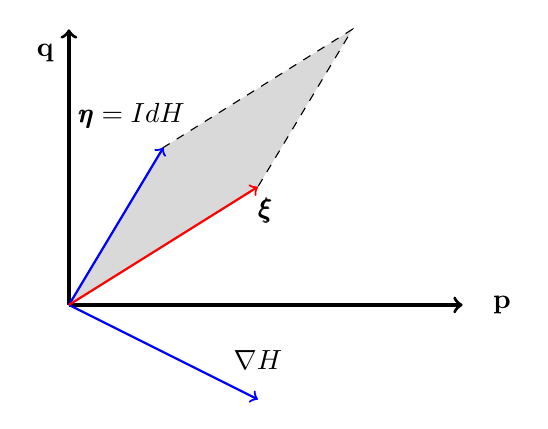
\begin{tikzpicture}
      % q axis
      \draw [very thick, ->] (0,0) -- (0,3.5);
      \node[](q) at (-0.3, 3.2){$\mathbf q$};

      % p axis
      \draw [very thick, ->] (0,0) -- (5,0);
      \node[](p) at (5.5, 0){$\mathbf p$};

      % the parallelogram
      \draw [dashed, fill=gray!30!white] (0, 0) -- (1.2, 2) -- (3.6, 3.5) -- (2.4, 1.5) -- cycle;

      % dH
      \draw [thick, ->, blue] (0, 0) -- (2.4, -1.2);
      \node[](dH) at (2.4, -0.7){$\nabla H$};

      % eta = IdH
      \draw [thick, ->, blue] (0, 0) -- (1.2, 2);
      \node[](IdH) at (0.8, 2.4){$\pmb\eta = I dH$};

      % xi
      \draw [thick, ->, red] (0, 0) -- (2.4, 1.5);
      \node[](eta) at (2.5, 1.2){$\pmb\xi$};
    \end{tikzpicture}
    \caption*{Illustration of $\omega^2(\pmb\xi, \pmb\eta) = (\pmb\xi, \nabla H)$.
    The area spanned by $\pmb\xi$ and $\pmb\eta = IdH$ is equal
    to the projection of $\nabla H$ on $\pmb \xi$.}
  \end{figure*}
    \note{$\omega^2(\pmb\xi, \pmb\eta) = \omega^1_{\pmb\eta}(\pmb\xi)
      = \omega^1_{IdH}(\pmb\xi) = (\pmb\xi, I^{-1} IdH)
    = dH(\pmb\xi)$.}
  Thus,
  $$
  \int_{J\gamma}\omega^2 = \int_0^\tau
  \left(
    \int_{g^t\tau} dH
  \right) dt.
  $$
  \note{$\int_0^1 \omega^2(\pmb\xi, \pmb\eta) \, ds
    = \int_0^1 dH(\pmb\xi) \, ds = \int_0^1 dH(\pmb\xi \, ds).$
    But $\pmb\xi = \frac{ \partial f' } { \partial s }
    = g^t \frac{ d f }{ d s } \rightarrow
    \pmb\xi\, ds = g^t \, df = d(g^t f)$,
    So
    $\int_0^1 dH(\pmb\xi ds) = \int dH(d g^t f) = \int_{g^t\gamma} dH.$
  }
\end{proof}


\begin{cor*}
  If the chain $\gamma$ is closed ($\partial \gamma = 0$)
  then $\int_{J\gamma} \omega^2 = 0$.

\end{cor*}

\begin{proof}
  $\int_\gamma dH = \int_{\partial \gamma} H = 0.$

  \note{
    $\int_{J\gamma} \omega^2 = \int_0^\tau \int_{g^t\gamma} dH \, dt
    = \int_0^\tau dt \int_{\partial(g^t \gamma)} H
    = \int_0^\tau dt \int_{g^t\partial\gamma} H = 0.$
  }
\end{proof}

\begin{proof}[Proof of the theorem.]
  We consider any 2-chain $c$. We have
  $$
  0 \stackrel{1}{=} \int_{Jc} d\omega^2
  \stackrel{2}{=} \int_{\partial Jc} \omega^2
  \stackrel{3}{=}
  \left(
    \int_{g^\tau c}
    -\int_{c}
    -\int_{J\partial c}
  \right)
  \omega^2
  \stackrel{4}{=}
  \left(
    \int_{g^\tau c}
    -\int_{c}
  \right)
  \omega^2.
  $$
  (1 since $\omega^2$ is closed, 2 by Stokes formula,
  3 by formula \eqref{eq:H_homotopy},
  4 by the corollary above with $\gamma = \partial c$).
  Thus the integrals of the form $\omega^2$
  on any chain $c$ and on its image $g^\tau c$ are the same.
\end{proof}


% subsection B
\subsection{Integral invariants}

Let $g:M\rightarrow M$ be a differentiable map.

\begin{defn*}
  A differential $k$-form $\omega$ is called an \emph{integral invariant}
  of the map $g$ if the integrals of $\omega$ on
  any $k$-chain $c$ and on its image under $g$ are the same:
  $$
  \int_{gc}\omega = \int_c \omega.
  $$
\end{defn*}

\begin{ex*}
  If $M = \mathbb{R}^2$ and $\omega^2 = dp \wedge dq$ is the area element,
  then $\omega^2$ is an integral invariant of any map $g$
  with jacobian $1$.
\end{ex*}

\begin{prob*}
  Show that a form $\omega^k$ is an integral invariant
  of a mapping if and only if $g^*\omega^k = \omega^k$.
\end{prob*}

\begin{prob*}
  Show that if the forms $\omega^k$ and $\omega^l$
  are integral invariants of the map,
  then the form $\omega^k \wedge \omega^l$
  is also an integral invariant of $g$.

  \answer{
    It follows from Problem \ref{prob:fstar_exprod} in Sec. 33.
    $$
    \begin{aligned}
    \int_{gc} (\omega^k \wedge \omega^l)
    &=
    \int_{c} (\omega^k \wedge \omega^l)(g\pmb\xi_1, \dots, g\pmb\xi_{k+l})
    =
    \int_{c} g^*(\omega^k \wedge \omega^l)(\pmb\xi_1, \dots, \pmb\xi_{k+l})
    \\
    &=\int_{c} (g^*\omega^k \wedge g^*\omega^l)(\pmb\xi_1, \dots, \pmb\xi_{k+l})
    =\int_{c} (\omega^k \wedge \omega^l)(\pmb\xi_1, \dots, \pmb\xi_{k+l}).
    \end{aligned}
    $$
  }
\end{prob*}

The theorem in subsection A can be reformulated as follows.

\begin{thm*}
  The form $\omega^2$ giving the symplectic structure
  is an integral invariant of a hamiltonian phase flow.
\end{thm*}

We now consider the exterior powers of $\omega^2$,
$$
(\omega^2)^2 = \omega^2 \wedge \omega^2,
\quad
(\omega^2)^3 = \omega^2 \wedge \omega^2 \wedge \omega^2,
\dots
$$

\begin{cor*}
  Each of the forms $(\omega^2)^2$, $(\omega^2)^3$, $(\omega^2)^4$, \dots
  is an integral invariant of a hamiltonian phase flow.
\end{cor*}

\begin{prob*}
Suppose that the dimension of the symplectic manifold
$(M^{2n}, \omega^2)$ is $2n$,
show that $(\omega^2)^k = 0$ for $k > n$,
and that $(\omega^2)^n$ is a nondegenerate $2n$-form on $M^{2n}$.
\end{prob*}

We define a volume element on $M^{2n}$ using $(\omega^2)^n$.
Then, a hamiltonian phase flow preserves volume,
and we obtain Liouville's theorem from the corollary above.

\begin{ex*}
  Consider the symplectic coordinate space
  $M^{2n} = \mathbb R^{2n} = \{(\mathbf p, \mathbf q)\}$,
  $\omega^2 = d\mathbf p \wedge d\mathbf q = \sum dp_i \wedge dq_i$.
  In this case the form $(\omega^2)^k$ is proportional to the form
  $$
  \omega^{2k} = \sum_{i_1 < \dots < i_k}
  dp_{i_1} \wedge \dots \wedge dp_{i_k} \wedge
  dq_{i_1} \wedge \dots \wedge dq_{i_k}.
  $$
  The integral of $\omega^{2k}$ is equal to the sum of
  the oriented volumes of projections on to the coordinate planes
  $(p_{i_1}, \dots, p_{i_k}, q_{i_1}, \dots, q_{i_k})$.
\end{ex*}

The map
$g: \mathbb R^{2n} \rightarrow \mathbb R^{2n}$
is called \emph{canonical} if it has $\omega^2$ as an integral invariant.
A canonical map is generally called a \emph{canonical transformation}.
Each of the forms $\omega^4, \omega^6, \dots, \omega^{2n}$
is an integral invariant of every canonical transformation.
Therefore, \emph{under a canonical transformation,
  the sum of the oriented areas of projections onto the coordinate planes
  $(p_{i_1}, \dots, p_{i_k}, q_{i_1}, \dots, q_{i_k})$,
  $1 \le k \le n$, is preserved}.
In particular, \emph{canonical transformations preserve volume}.

The hamiltonian phase flow given by the equations
$\dot{\mathbf p} = -\partial H/\partial \mathbf q$,
$\dot{\mathbf q} = \partial H/\partial \mathbf p$
consists of canonical transformations $g^t$.

The integral invariants considered above are also called
\emph{absolute integral invariants}.

\begin{defn*}
  A differential $k$-form is called a
  \emph{relative integral invariant} of the map
  $g: M \rightarrow M$ if
  $\int_{gc} \omega = \int_c \omega$
  for every \emph{closed} $k$-chain $c$.
\end{defn*}

\begin{thm*}
  Let $\omega$ be a relative integral invariant of a map $g$.
  Then $d\omega$ is an absolute integral invariant of $g$.
\end{thm*}

\begin{proof}
  Let $c$ be a $k+1$-chain. Then
  $$
  \int_c d\omega \stackrel{1}{=}
  \int_{\partial c} \omega
  \stackrel{2}{=}
  \int_{g\partial c} \omega
  \stackrel{3}{=}
  \int_{\partial gc} \omega
  \stackrel{4}{=}
  \int_{gc} d\omega.
  $$
  (1 and 4 are by Stokes' formula,
  2 by the definition of relative invariant,
  and 3 by the definition of boundary).
\end{proof}


\begin{ex*}
  A canonical map $g:\mathbb R^{2n} \rightarrow \mathbb R^{2n}$
  has the 1-form
  $$
  \omega^1 = \mathbf p \, d\mathbf q = \sum_{i = 1}^n p_i \, dq_i
  \mbox{ as a relative integral invariant.}
  $$
  \note{This is more like a converse of the above theorem,
  not a deduction.}
  In fact, every closed chain $c$ on $\mathbb R^{2n}$
  is the boundary of some chain $\sigma$
  \note{Recall the cone construction in Sec. 36},
  and we find
  $$
  \int_{gc} \omega^1
  \stackrel{1}{=}
  \int_{g\partial \sigma} \omega^1
  \stackrel{2}{=}
  \int_{\partial g\sigma} \omega^1
  \stackrel{3}{=}
  \int_{g\sigma} d\omega^1
  \stackrel{4}{=}
  \int_{\sigma} d\omega^1
  \stackrel{5}{=}
  \int_{\partial \sigma} \omega^1
  \stackrel{6}{=}
  \int_{c} \omega^1.
  $$
  (1 and 6 are by definition of $\sigma$,
  2 by definition of $\partial$,
  3 and 5 by Stokes' formula,
  and 4 since $g$ is canonical and
  $d\omega^1 = d(pdq) = dp \wedge dq = \omega^2$).
\end{ex*}


\begin{prob*}
  Let $d\omega^k$ be an absolute integral invariant of the map
  $g: M \rightarrow M$. Does it follow that $\omega^k$ is a
  relative integral invariant?
\end{prob*}

\begin{ans*}
  No, if there is a closed $k$-chain on $M$ which is not a boundary.
  \note{
  We still have
  $
  \int_{g\partial c} \omega^k =
  \int_{gc} d\omega^k =
  \int_c d\omega^k =
  \int_{\partial c} \omega^k.
  $
  The problem is that there are closed chains $\gamma$ that cannot be
  written as $\partial c$, like an equator of the torus, $T^2$,
  which will fail $\omega^k$.
  }
\end{ans*}


% subsection C
\subsection{The law of conservation of energy}

\begin{thm*}
  The function $H$ is a first integral of the hamiltonian phase flow
  with hamiltonian function $H$.
\end{thm*}

\begin{proof}
  The derivative of $H$ in the direction of a vector $\pmb\eta$
  is equal to the value of $dH$ on $\pmb\eta$.
  By definition of the hamiltonian field
  $\pmb\eta = IdH$ we find
  $$
  dH(\pmb\eta) = \omega^2(\pmb\eta, IdH)
  = \omega^2(\pmb\eta, \pmb\eta) = 0.
  $$
\end{proof}

\begin{prob*}
  Show that the 1-form $dH$ is an integral invariant
  of the phase flow with hamiltonian function $H$.

\answer{
  $$
  \left( \int_{g\gamma} - \int_{\gamma} \right) dH
  =
  \int_{\partial(Jc) } dH + \int_{J\partial c} dH
  =
  \int_{Jc} ddH + \int_0^1 dH(\pmb\eta) \, dt
  = 0 + 0 = 0.
  $$
}
\end{prob*}


% section 39
\section{The Lie algebra of vector fields}


Every pair of vector fields on a manifold determines a new vector field,
called their Poisson bracket\footnote{Or Lie bracket}.
%
The Poisson bracket operation makes the vector space of
infinitely differentiable vector fields
on a manifold into a Lie algebra.

% subsection 39A
\subsection{Lie algebras}

One example of a Lie algebra is a three-dimensional oriented euclidean
vector space equipped with the operation of vector multiplication.
%
The vector product is bilinear, skew symmetric, and satisfies the
\emph{Jacobi identity}
  $$
    [[A, B], C] + [[B, C], A] + [[C, A], B].
  $$

\note{The Jacobi identity for the vector product reads
$$
\mathbf{
  (A \times B) \times C
+ (B \times C) \times A
+ (C \times A) \times B
= 0}.
$$
To show this, we recall
$\mathbf{[(A \times B) \times C]}_k = \epsilon_{ijk}\epsilon_{imn} A_m B_n C_j
= (\delta_{jm}\delta_{kn} - \delta_{jn}\delta_{mk}) A_m B_n C_j
= C_j A_j B_k - B_j C_j A_k
= \mathbf{[(C\cdot A) \, B - (B\cdot C) A]}_k$;
similarly
$\mathbf{
  (B\times C)\times A
=(A\cdot B) \, C - (C \cdot A) \, B}$,
and
$\mathbf{(C\times A)\times B
=(B\cdot C) \, A - (A \cdot B) \, C}$.
The three sum to $0$.
Poisson bracket can be viewed as a generalization of
the idea of vector cross product in higher spaces.
}

\begin{defn*}
  A \emph{Lie algebra} is a vector space $L$,
  together with a bilinear skew-symmetric operation
  $L\times L \rightarrow L$ which satisfies the Jacobi identity.

  The operation is usually denoted by square brackets
  and called the commutator.
\end{defn*}

\begin{prob*}
  Show that the set of $n\times n$ matrices becomes a Lie algebra
  if we define the commutator by $[A, B] = AB - BA$.

  \answer{The bilinearity is easy. Let us verify the Jacobi identity.
    After expansion, each term on the left-hand side is a product of
    three matrices.  Let us collect all terms that end with $C$:
    $[[A, B], C]$ contributes $[A, B] C$;
    $[[B, C], A]$ contributes $-ABC$ through $-A[B,C]$,
    $[[C, A], B]$ contributes $BAC$ through $-B[C,A]$,
    and
    $$[A, B] C - ABC + BAC = 0.$$
    By the cyclic symmetry, the same holds for terms end with $A$ or $B$,
    so the Jacobi identity is satisfied.
  }
\end{prob*}


% subsection B
\subsection{Vector fields and differential operators}

Let $M$ be a smooth manifold and $\mathbf A$ a smooth vector field on $M$:
at every point $\mathbf x \in M$ we are given a tangent vector
$\mathbf{ A(x) } \in TM_{\mathbf x}$.
With every such vector field we associate the following two objects:
\begin{enumerate}
  \item
    \emph{The one-parameter group of diffeomorphisms} or \emph{flow}
    of $A^t: M \rightarrow M$ for which $\mathbf A$ is the velocity vector field
    (Figure 168):\footnote{
    By theorems of existence, uniqueness and differentiability
    in the theory of ordinary differential equations,
    the group $A^t$ is defined if the manifold is compact.
    In the general case, the maps $A^t$ are defined only in a neighborhood
    of $\mathbf x$ and only for small $t$; this is enough
    for the following constructions.
    \note{A subset is
      ``compactness'' if it is \emph{closed}
      (containing all its limit points)
      and \emph{bounded} (having all its points lie
      within some fixed distance of each other).
      Examples of compact manifolds include
      the circle and $n$-dimensional sphere and torus.
    }
    }
    $$
    \frac{d}{dt}\bigg|_{t = 0} A^t \mathbf x = \mathbf{ A(x) }.
    $$

    \begin{figure}
      \centering
      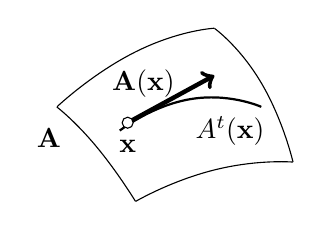
\begin{tikzpicture}
        % parallelogram
        \draw [] plot [smooth, tension=1]
        coordinates{(1, 0) (2, 0.4) (3, 0.5)};
        \draw [] plot [smooth, tension=1]
          coordinates{(3, 0.5) (2.6, 1.5) (2, 2.2)};
        \draw [] plot [smooth, tension=1]
          coordinates{(2, 2.2) (1, 1.9) (0, 1.2)};
        \draw [] plot [smooth, tension=1]
          coordinates{(0, 1.2) (0.5, 0.7) (1, 0)};

        % A
        \node [] at (-0.1, 0.8) {$\mathbf A$};

        % x
        \node [] at (0.9, 0.7) {$\mathbf x$};

        % A^t(x)
        \node [] at (2.2, 0.9) {$A^t(\mathbf x)$};

        % A(x)
        \node [] at (1.1, 1.5) {$\mathbf{ A(x)}$};
        % the curve A^t(x)
        \draw [thick] plot [smooth, tension=1]
          coordinates{(0.8, 0.9) (1.7, 1.3) (2.6, 1.2)};

        % the tangent vector
        \draw [ultra thick, ->] (0.9, 1.0) -- (2.0, 1.6);

        \draw [fill=white] (0.9, 1.0) circle (0.07);

      \end{tikzpicture}
      \label{fig:flow_vecfield}
      \caption{The group of diffeomorphism given by
      a vector field}
    \end{figure}

  \item
    The first-order differential operator $L_\mathbf{A}$.
    We refer here to the differentiation of functions
    in the direction of the field $\mathbf A$:
    for any function $\varphi: M \rightarrow \mathbb F$,
    the \emph{derivative in the direction of $\mathbb A$}
    is a new function $L_{\mathbf A} \varphi$,
    whose value at a point $\mathbf x$ is
    $$
    (L_{\mathbf A}\varphi) (\mathbf x)
    =
    \frac{d}{dt}\bigg|_{t = 0} \varphi(A^t\mathbf x).
    $$

\end{enumerate}

\begin{prob*}
  Show that the operator $L_\mathbf{A}$ is linear:
  $$
  L_\mathbf{A}(\lambda_1 \varphi_1 + \lambda_2 \varphi_2)
  =
  \lambda_1 L_\mathbf{A}\varphi_1
  +
  \lambda_2 L_\mathbf{A}\varphi_2
  \qquad
  (\lambda_1, \lambda_2 \in \mathbb{R}).
  $$
  Also, prove the Leibniz's formula
  $
  L_\mathbf{A}(\varphi_1\varphi_2)
  = \varphi_1 L_\mathbf{A} \varphi_2 + \varphi_2 L_\mathbf{A} \varphi_1.
  $

  \answer{
    For the linearity:
    $$
    \begin{aligned}
    L_\mathbf{A}(\lambda_1 \varphi_1 + \lambda_2 \varphi_2)
    &=
    \frac{d}{dt}\bigg|_{t = 0}
    \left[
    \lambda_1 \varphi_1(A^t\mathbf x)
    +
    \lambda_2 \varphi_2(A^t\mathbf x)
    \right]
    \\
    &=
    \lambda_1
    \frac{d}{dt}\bigg|_{t = 0}
    \varphi_1(A^t\mathbf x)
    +
    \lambda_2
    \frac{d}{dt}\bigg|_{t = 0}
    \varphi_2(A^t\mathbf x) \\
    &=
    \lambda_1
    (L_{\mathbf A}\varphi_1) (\mathbf x)
    +
    \lambda_2
    (L_{\mathbf A}\varphi_2) (\mathbf x).
    \end{aligned}
    $$

    For the Leibniz's formula:
    $$
    \begin{aligned}
    L_\mathbf{A}(\varphi_1 \varphi_2)
    &=
    \frac{d}{dt}\bigg|_{t = 0}
    \varphi_1(A^t\mathbf x)
    \varphi_2(A^t\mathbf x)
    \\
    &=
    \varphi_1(\mathbf x)
    \frac{d}{dt}\bigg|_{t = 0}
    \varphi_2(A^t\mathbf x)
    +
    \varphi_2(\mathbf x)
    \frac{d}{dt}\bigg|_{t = 0}
    \varphi_1(A^t\mathbf x) \\
    &=
    \varphi_1(\mathbf x)
    (L_{\mathbf A}\varphi_2) (\mathbf x)
    +
    \varphi_2(\mathbf x)
    (L_{\mathbf A}\varphi_1) (\mathbf x).
    \end{aligned}
    $$
  }
\end{prob*}

\begin{ex*}
  Let $(x_1, \dots, x_n$ be local coordinates on $M$.
  In this coordinate system the vector $\mathbf{ A(x) }$
  is given by its components
  $(A_1(\mathbf x), \dots, A_n(\mathbf x))$;
  the flow $A^t$ is given by the system of differential equations
  $$
  \dot x_1 = A_1(\mathbf x), \dots
  \dot x_n = A_n(\mathbf x)
  $$
  and, therefore, the derivative of
  $\varphi = \varphi(x_1, \dots, x_n)$
  in the direction $\mathbf A$ is
  $$
  L_\mathbf{A} \varphi = A_1 \frac{\partial \varphi}{\partial x_1}
  + \dots A_n \frac{ \partial \varphi }{ \partial x_n }.
  $$
  We could say that in the coordinates $(x_1, \dots, x_n)$
  the operator $L_\mathbf{A}$ has the form
  $$
  L_\mathbf{A} = A_1 \frac{\partial }{\partial x_1}
  + \dots + A_n \frac{ \partial }{ \partial x_n}.
  $$
  This is the general form of a first-order linear differential operator
  on coordinate space.
\end{ex*}

\begin{prob*}
  Show that the correspondences between vector fields $\mathbf A$,
  flows $A^t$, and differentiations $L_\mathbf{A}$ are one-to-one.

  \answer{
    The correspondence between the vector field $\mathbf A$
    and the differentiations $L_\mathbf{A}$ are apparent
    from the above example.
    For $\mathbf A$ and the flow, we first note that
    by definition the vector field $\mathbf{ A(x)}$ is determined by the flow.
    Conversely, we can trace the flow
    by following the vector field $\mathbf{ A(x) }$,
    That is,
    for a sufficiently small $\Delta t$,
    the flow approximately satisfies the recurrence relation
    $$
    A^t(\mathbf x) \approx
    A^{t-\Delta t}(\mathbf x + \Delta t \mathbf{A(x)})
    =
    A^{t-\Delta t} (1 + \Delta t \mathbf{A})\mathbf x.
    $$
    Or,
    $$
    A^t(\mathbf x)
    =
    \lim_{n\rightarrow \infty}
    \left(1 + \frac{t}{n} \mathbf{A}\right)^{n} \mathbf x.
    =
    \exp(t\mathbf{A}) \, \mathbf x.
    $$
    which means the flow is completely determined by the vector field.
  }
\end{prob*}

% subsection C
\subsection{Poisson bracket of vector fields}




% section 40
\section{The Lie algebra of hamiltonian functions}

\begin{figure}
  \centering
 \begin{tikzpicture}
    \draw (-1,0) to[bend left] (1,0);
    \draw (-1.2,.1) to[bend right] (1.2,.1);
    \draw[rotate=0] (0,0) ellipse (100pt and 50pt);
  \end{tikzpicture}
\end{figure}

\section{Symplectic geometry}

\section{Parametric resonance in systems with many degrees of freedom}

\section{A symplectic atlas}

\chapter{Canonical formalism}

\section{The integral invariant of Poincar\'e-Cartan}

\section{Applications of the integral invariant of Poincar\'e-Cartan}

\section{Huygens' principle}

\section{The Hamilton-Jacobi method for integrating Hamilton's canonical equations}

\section{Generating functions}

\chapter{Introduction to perturbation theory}

\section{Integrable systems}

\section{Action-angle variables}

\section{Averaging}

\section{Averaging of perturbations}

\appendix
\renewcommand{\thechapter}{\arabic{chapter}}

\chapter{Riemannian curvature}

\chapter{Geodesics of left-invariant metrics on Lie groups and
the hydrodynamics of ideal fluids}

\chapter{Symplectic structures on algebraic manifolds}

\chapter{Contact structures}

\chapter{Dynamical systems with symmetries}

\chapter{Normal forms of quadratic hamiltonians}

\chapter{Normal forms of hamiltonian systems near stationary points
and closed trajectories}

\chapter{Theory of perturbations of conditionally periodic motion,
and Kolmogorov's theorem}

\chapter{Poincar\'e's geometric theorem, its generalizations and
applications}

\chapter{Multiplicities of characteristic frequencies, and ellipoids
depending on parameters}

\chapter{Short wave asymptotics}

\chapter{Lagrangian singularities}

\chapter{The Korteweg-de Vries equation}

\chapter{Poisson structures}

\chapter{On elliptic coordinates}

\chapter{Singularities of ray systems}

\end{document}
